% Provenance (never printed): see sources/outline_sources.md (Year 3:
% concordia and discordia; 40Ar/39Ar step heating; Sm-Nd model ages;
% cosmogenic nuclides; fission tracks and (U-Th)/He). Brief:
% sources/book5/BRIEFS.md, ch. 13. Curves from figdata/bachelor-3/
% concordia.py, arar_spectrum.py, model_ages.py, cosmogenic.py. Exercise and
% problem values in the Book 5 scratch calculator calc/ch13.py. The zircons,
% the biotite spectrum, the Nd sample and the helium ages of the Varden
% granite are invented, consistent with the Year 1 volume's granite of 310 Ma.
\chapter{高级地质年代学}\label{ch:b3:advanced-geochronology}

一颗长十分之一毫米的锆石晶体，自其花岗岩结晶以来，
一直运行着两只“时钟”：铀-238 衰变为铅-206，
铀-235 衰变为铅-207。两只“时钟”一致时，年龄便
确凿无疑。两者不一致时，这种不一致本身即可用于定年：
晶体在后来的某次事件中丢失了部分铅，将两只“时钟”放在一起读取，
便可同时得到花岗岩的年龄与该事件的年龄。本章
将同时读取多种“时钟”：铀和铅、氩、钕、
裂变径迹与氦，以及宇宙射线产生的稀有原子，
并说明每种年龄的可信程度。

\begin{recall}
放射性衰变、年龄方程、等时线及其初始比值、
最小二乘直线、分支衰变、钾–氩年龄、封闭
温度与冷却年龄均见于本科一年级分册中关于
放射性测年的一章；\omterm{def:b3:advanced-geochronology:cosmogenic}{宇宙成因核素}的稳态侵蚀公式见于
其侵蚀与搬运一章。球粒陨石均一储库、
ε 表示法与亏损地幔见于本科二年级分册中的
同位素地球化学一章；热电离质谱法和多接收质谱法
见于其关于野外与实验室方法的一章。\omterm{def:b3:orogenic-wedges:thermochronology}{热年代学}与
\omterm{def:b3:orogenic-wedges:age-elevation}{年龄–高程关系}见于\cref{ch:b3:orogenic-wedges}。
\end{recall}

\section{铀、铅与谐和线}\label{sec:b3:advanced-geochronology:upb}

铀有两种长寿命同位素。铀-238 经一系列短寿命子体衰变为铅-206，
其衰变常数为 $\lambda_{238} =
\qty{1.55125e-10}{\text{年}^{-1}}$；铀-235 衰变为铅-207，其衰变常数为 $\lambda_{235}
= \qty{9.8485e-10}{\text{年}^{-1}}$，快六倍。二者现今的比值为
$^{235}\mathrm{U}/^{238}\mathrm{U} = 0.0072567$，或 $^{238}\mathrm{U}/^{235}\mathrm{U}
= 137.8$，在所有陆地岩石中都相同。锆石 $\mathrm{ZrSiO_4}$ 结晶时
吸纳大量铀而几乎不含铅，并且抗风化，
能经受变质作用而保存下来：其铅几乎全部为放射成因。
% ledger: amherst:constants, tulane:upb-zircon

记 $x = {}^{207}\mathrm{Pb}^*/{}^{235}\mathrm{U}$ 与 $y =
{}^{206}\mathrm{Pb}^*/{}^{238}\mathrm{U}$ 为放射成因铅与其母体的现今比值。
每个比值各给出一个年龄：$t_{206} = \ln(1 + y)/\lambda_{238}$
和 $t_{207} = \ln(1 + x)/\lambda_{235}$。

\begin{definition}[谐和线、不一致线、交点、特拉–瓦瑟堡图]
\label{def:b3:advanced-geochronology:concordia}
\emph{谐和线}\index{谐和线}是 $(x, y)$ 平面上的一条曲线，
该曲线上两个铀–铅年龄相等。\emph{不一致线}\index{不一致线}
是一条直线，同一群体晶体中不一致的分析点
沿此直线排列；其与谐和线的交点为
\emph{上交点}\index{上交点}（较老者）和
\emph{下交点}\index{下交点}（较年轻者）。
\emph{特拉–瓦瑟堡图}\index{特拉–瓦瑟堡图}以
$X = {}^{238}\mathrm{U}/{}^{206}\mathrm{Pb}^*$ 对 $Y =
{}^{207}\mathrm{Pb}^*/{}^{206}\mathrm{Pb}^*$ 作图。
\end{definition}

\begin{theorem}[谐和线]\label{thm:b3:advanced-geochronology:concordia}
一颗自形成以来对铀和铅始终保持封闭的晶体，形成于距今
$t$ 时，其点位于
\[
C(t) = \bigl(e^{\lambda_{235}t} - 1,\; e^{\lambda_{238}t} - 1\bigr).
\]
随 $t$ 增大，曲线相对于 $x$ 上升得越来越慢：其斜率
$\mathrm dy/\mathrm dx = (\lambda_{238}/\lambda_{235})\,e^{(\lambda_{238} -
\lambda_{235})t}$，斜率在原点处为 $\lambda_{238}/\lambda_{235} = 0.1575$，
随之递减，故\omterm{def:b3:advanced-geochronology:concordia}{谐和线}凹向 $x$ 轴。
\end{theorem}

\begin{proof}
对每种母体而言，剩余母体原子所对应的放射成因子体数为
$e^{\lambda t} - 1$，即本科一年级分册中的年龄方程。对两坐标分别关于 $t$ 求导，
再相除即得斜率；由于
$\lambda_{235} > \lambda_{238}$，斜率随 $t$ 减小。
\end{proof}

铅是一种大离子，很难嵌入锆石晶格。在晶体的
因自身放射性而受损的部分，铅可在后来的某次
加热或流体循环事件中逸出。
% ledger: tulane:upb-zircon

\begin{theorem}[阶段性铅丢失给出弦]\label{thm:b3:advanced-geochronology:discordia}
一颗形成于距今 $t_1$ 时的晶体，在距今 $t_2$ 时丢失了其
放射成因铅的比例 $f$，其余时间保持封闭，则今日位于
\[
(1 - f)\,C(t_1) + f\,C(t_2),
\]
位于\omterm{def:b3:advanced-geochronology:concordia}{谐和线}上 $t_1$ 与 $t_2$ 两点连线所成的弦上。丢失比例不同的
晶体均落在这条弦上，构成一条\omterm{def:b3:advanced-geochronology:concordia}{不一致线}，其\omterm{def:b3:advanced-geochronology:concordia}{上交点}为
$t_1$，\omterm{def:b3:advanced-geochronology:concordia}{下交点}为 $t_2$。
\end{theorem}

\begin{proof}
取一个衰变体系，衰变常数为 $\lambda$，按今日存在的母体原子计数。
距今 $t_2$ 时母体原子有 $e^{\lambda t_2}$ 个，
其放射成因子体为 $e^{\lambda t_2}(e^{\lambda(t_1 - t_2)} - 1) =
e^{\lambda t_1} - e^{\lambda t_2}$。事件之后余下 $(1 - f)(e^{\lambda t_1} -
e^{\lambda t_2})$；此后母体又多生成了 $e^{\lambda t_2} - 1$ 个。
二者之和为 $(1 - f)(e^{\lambda t_1} - 1) + f(e^{\lambda t_2} - 1)$。两种铅同位素
的化学性质相似，因此 $f$ 对两者相同，两个坐标
合并即得所述之点。
\end{proof}

\begin{omfigure}
\begin{tikzpicture}
\begin{groupplot}[group style={group size=2 by 1, horizontal sep=1.7cm},
  omrecord, width=0.47\linewidth, height=0.42\linewidth, title style={font=\small},
  tick label style={font=\scriptsize}, label style={font=\small}]
\nextgroupplot[title={(a) 谐和线图},
  xlabel={$^{207}\mathrm{Pb}^*/^{235}\mathrm{U}$}, ylabel={$^{206}\mathrm{Pb}^*/^{238}\mathrm{U}$},
  xmin=0.04, xmax=0.44, ymin=0.006, ymax=0.06,
  xtick={0.1,0.2,0.3,0.4}, xticklabels={0.1,0.2,0.3,0.4},
  ytick={0.01,0.02,0.03,0.04,0.05}, yticklabels={0.01,0.02,0.03,0.04,0.05},
  scaled ticks=false]
% computed in figdata/bachelor-3/concordia.py
\addplot[black, thick] table[x=xw, y=yw] {figdata/out/bachelor-3-concordia-curve.dat};
\addplot[black, only marks, mark=*, mark size=1.4pt, nodes near coords={\scriptsize\pgfmathprintnumber[fixed, precision=0]{\pgfplotspointmeta}},
  point meta=explicit, nodes near coords align={anchor=south east},
  restrict expr to domain={\thisrow{t}}{100:350}]
  table[x=xw, y=yw, meta=t] {figdata/out/bachelor-3-concordia-ticks.dat};
\addplot[omDef, thick, densely dashed] table[x=x, y=y] {figdata/out/bachelor-3-concordia-line.dat};
\addplot[red!70!black, only marks, mark=diamond*, mark size=2pt] table[x=x, y=y] {figdata/out/bachelor-3-concordia-zircons.dat};
\nextgroupplot[title={(b) 特拉–瓦瑟堡图},
  xlabel={$^{238}\mathrm{U}/^{206}\mathrm{Pb}^*$}, ylabel={$^{207}\mathrm{Pb}^*/^{206}\mathrm{Pb}^*$},
  xmin=15, xmax=75, ymin=0.0465, ymax=0.0535,
  ytick={0.047,0.049,0.051,0.053}, yticklabels={0.047,0.049,0.051,0.053},
  scaled ticks=false]
\addplot[black, thick] table[x=xtw, y=ytw] {figdata/out/bachelor-3-concordia-curve.dat};
\addplot[black, only marks, mark=*, mark size=1.4pt, nodes near coords={\scriptsize\pgfmathprintnumber[fixed, precision=0]{\pgfplotspointmeta}},
  point meta=explicit, nodes near coords align={anchor=north east},
  restrict expr to domain={\thisrow{t}}{100:250}]
  table[x=xtw, y=ytw, meta=t] {figdata/out/bachelor-3-concordia-ticks.dat};
\addplot[omDef, thick, densely dashed] table[x=xtw, y=ytw] {figdata/out/bachelor-3-concordia-twline.dat};
\addplot[red!70!black, only marks, mark=diamond*, mark size=2pt] table[x=xtw, y=ytw] {figdata/out/bachelor-3-concordia-zircons.dat};
\end{groupplot}
\end{tikzpicture}

\par\smallskip{\small (a) 协和线，图中年龄以百万年为单位，
和同一花岗岩中的五颗虚构不一致锆石（红色；其误差
椭圆小于符号），它们沿一条\omterm{def:b3:advanced-geochronology:concordia}{不一致线}（虚线）排列，该线
在约 311 与 \qty{100}{\Ma} 处与协和线相交。(b) 同一批锆石及直线
在\omterm{def:b3:advanced-geochronology:concordia}{特拉–瓦瑟堡图}中的表示，其中\omterm{def:b3:advanced-geochronology:concordia}{不一致线}仍是
直线。}\label{fig:b3:advanced-geochronology:concordia}
\end{omfigure}
% ledger: amherst:constants

交点由 $a + b\,x(t) = y(t)$ 确定，这是关于 $t$ 的方程，
用牛顿法求解：令 $g(t) = e^{\lambda_{238}t} - 1 - a -
b(e^{\lambda_{235}t} - 1)$ 及 $g'(t) = \lambda_{238}e^{\lambda_{238}t} -
b\lambda_{235}e^{\lambda_{235}t}$，迭代 $t \leftarrow t - g/g'$，初值取
各交点附近的猜测值。实际应用中，结果有以下三条性质。
第一，\omterm{def:b3:advanced-geochronology:concordia}{上交点}只有在\omterm{def:b3:advanced-geochronology:concordia}{不一致线}与协和线相交的
夹角较大时才精确。如上图所示，年轻的\omterm{def:b3:advanced-geochronology:concordia}{不一致线}
几乎沿协和线延伸，其斜率的微小变化会使
交点大幅移动。第二，若铅丢失是近期发生的，$t_2 = 0$，则\omterm{def:b3:advanced-geochronology:concordia}{不一致线}
通过原点，所有晶体具有相同的
$^{207}\mathrm{Pb}^*/^{206}\mathrm{Pb}^*$ 比值，
\[
\frac{^{207}\mathrm{Pb}^*}{^{206}\mathrm{Pb}^*} = \frac{1}{137.8}\,
\frac{e^{\lambda_{235}t_1} - 1}{e^{\lambda_{238}t_1} - 1},
\]
由此可在不用铀的情况下得到 $t_1$，即铅–铅年龄。第三，协和图中的一条直线
$x = (y - a)/b$，在特拉–瓦瑟堡坐标中变为
$Y = (1 - aX)/(137.8\,b)$，仍是一条直线。\omterm{def:b3:advanced-geochronology:concordia}{特拉–瓦瑟堡
图}直接使用实测比值，无需由铀-238 换算铀-235，
而含普通铅、非放射成因且富含铅-207 的混合物，
其数据点落在一条直线上，该直线与 $Y$ 轴
相交于普通铅的比值处。

铀–铅年龄有两种测量方式。单颗晶体或晶体片段，
经部分溶解去除受损区后再溶解，
并分离其中的铅和铀，经
热电离质谱法测量，得到地质学中最精确的年龄。直径约数十
微米的斑点原位测量，用离子探针或激光
剥蚀，精度较低，但可沿一颗在
多次事件中生长的晶体逐带测量。

\begin{inthelab}[地质年代学实验室]
\begin{minipage}[t]{0.55\linewidth}\vspace{0pt}
锆石定年始于破碎的岩石，终于洁净的实验室。地质年代学家
按密度和磁性分选锆石，挑选最清晰的
晶体，在双目显微镜下观察并对其环带成像。
晶体先经部分溶解以去除受损区，然后
以已知同位素的稀释剂完全溶解，铀和铅
在微型树脂柱上分离，操作于经过滤的空气中，以防
尘埃中的铅混入。质谱仪测量同位素比值。氩样品
走另一条路线：先经反应堆照射，再经气体管路，激光逐步加热每一步，
氩在进入质谱仪前被净化。
\end{minipage}\hfill
\begin{minipage}[t]{0.42\linewidth}\vspace{0pt}
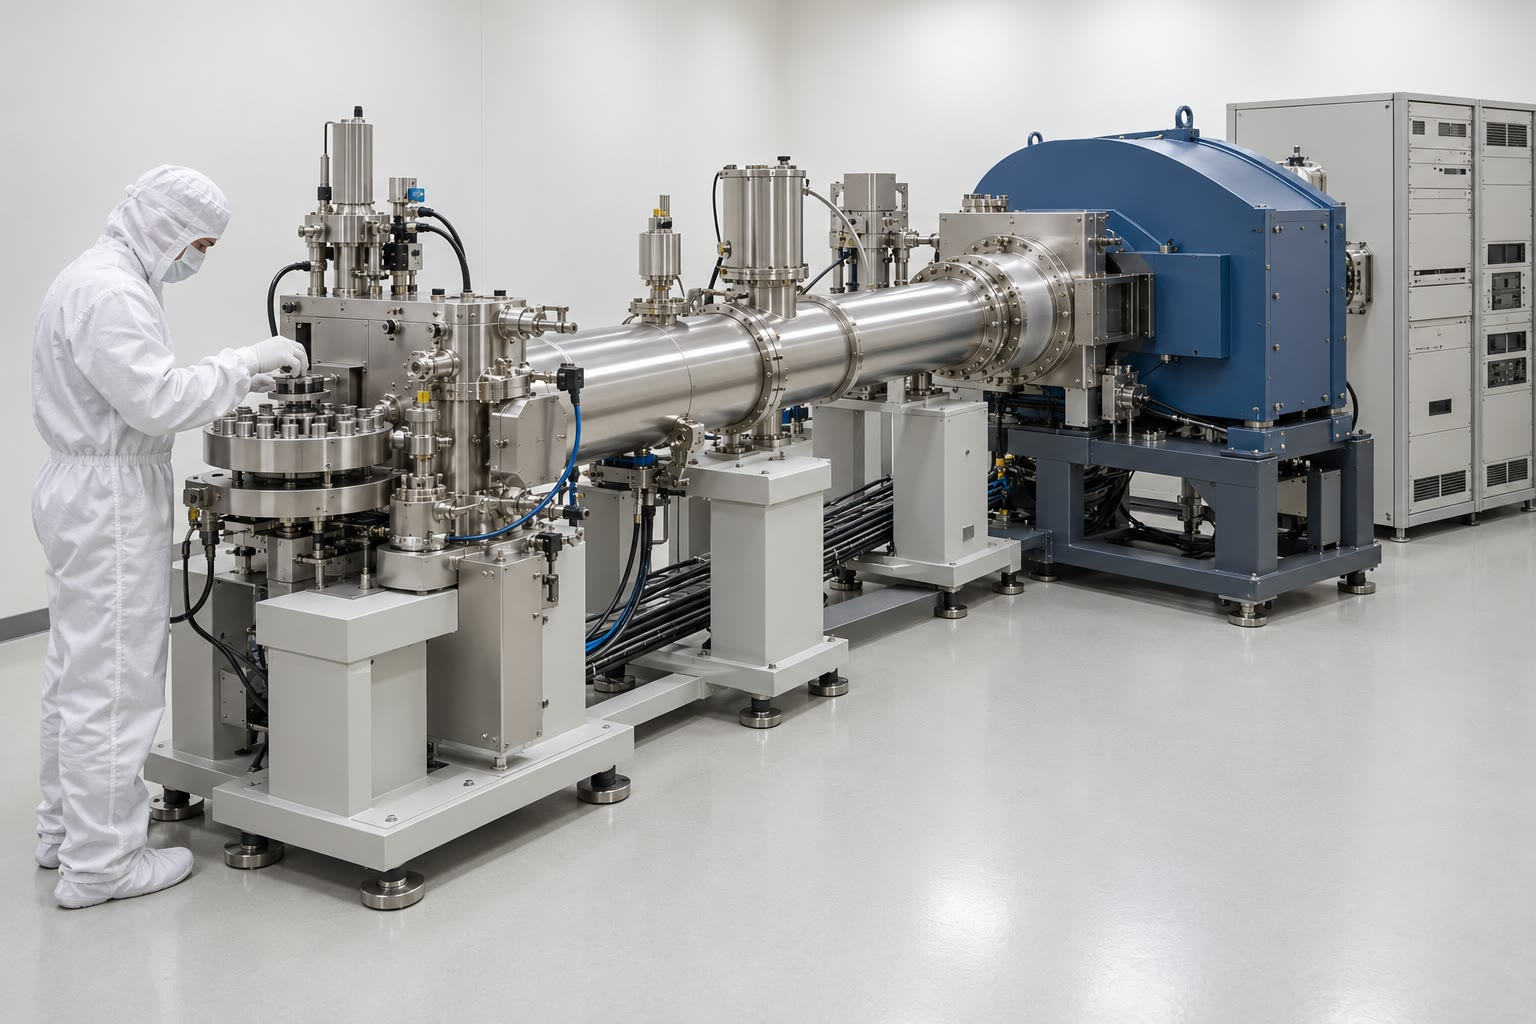
\includegraphics[width=\linewidth]{images/book5/ai/b3-mass-spec-lab.jpg}

{\scriptsize 洁净实验室中的质谱仪：样品转盘位于
左侧，飞行管与电磁铁（AI 生成
插图）。}
\end{minipage}
\end{inthelab}

\section{氩–氩定年}\label{sec:b3:advanced-geochronology:arar}

本科一年级分册中的钾–氩法在矿物的两份等份样中分别测量钾和
氩。氩–氩法只在一份等份样中测量氩，以同位素比值表示。样品
在核反应堆堆芯中受快中子照射，
其中反应 $^{39}\mathrm{K}(n,p)^{39}\mathrm{Ar}$ 使固定比例的钾-39
转化为氩-39，氩-39 可作为钾的代用指标。
一种已知年龄的矿物，即监测样，
与样品同被照射。
% ledger: nmgrl:arar, amherst:arar

\begin{definition}[氩–氩定年、J 因子、年龄谱、坪年龄]
\label{def:b3:advanced-geochronology:arar}
\emph{$^{40}\mathrm{Ar}/^{39}\mathrm{Ar}$ 定年}\index{氩–氩定年@$^{40}\mathrm{Ar}/^{39}\mathrm{Ar}$ 定年}
测定含钾矿物的年龄，方法是用比值 $R =
{}^{40}\mathrm{Ar}^*/{}^{39}\mathrm{Ar}_{\mathrm K}$ 为其放射成因氩-40 与
经中子照射由其钾生成的氩-39 之比。
某次照射的 \emph{J 因子}\index{J 因子}为 $J = (e^{\lambda
t_m} - 1)/R_m$，由已知年龄 $t_m$ 的监测样及其
实测比值 $R_m$，$\lambda$ 为钾-40 的总衰变常数。样品
按逐级升温脱气时，其\emph{年龄
谱}\index{年龄谱}以各步年龄对
累计释放的氩-39 比例作图。\emph{坪
年龄}\index{坪年龄}是相邻各步的加权平均年龄，这些步
在误差范围内相互一致，并释放了大部分氩-39。
\end{definition}

\begin{theorem}[氩–氩年龄]\label{thm:b3:advanced-geochronology:arar}
经监测样照射的样品，其年龄为
\[
t = \frac1\lambda\ln(1 + JR).
\]
\end{theorem}

\begin{proof}
放射成因氩为 $^{40}\mathrm{Ar}^* = (\lambda_e/\lambda)\,
{}^{40}\mathrm{K}\,(e^{\lambda t} - 1)$，据本科一年级
分册中的分支衰变。生成的氩-39 为 $^{39}\mathrm{Ar}_{\mathrm K} =
{}^{39}\mathrm{K}\,\Phi$，其中 $\Phi$ 汇集了中子剂量与
反应截面。因此 $R = (e^{\lambda t} - 1)/J$，其中 $J =
\lambda\,\Phi\,{}^{39}\mathrm{K}/(\lambda_e\,{}^{40}\mathrm{K})$。比值
$^{40}\mathrm{K}/^{39}\mathrm{K}$ 在所有钾中都相同，$\Phi$ 也
对并排照射的两个样品相同，因此 $J$ 对样品
与监测样都相同；由监测样的年龄和比值给出它，反解 $R$ 即得
$t$。
\end{proof}

常数与钾–氩法所用的相同，$\lambda =
\qty{5.543e-10}{\text{年}^{-1}}$。常用监测样是一种火山凝灰岩中的
透长石，其年龄定为 \qty{28.201}{\Ma}；监测样比值 $R_m = 1.3129$ 给出 $J =
0.01200$。大气氩，其 $^{40}\mathrm{Ar}/^{36}\mathrm{Ar} = 295.5$，
须以各步中实测的氩-36 扣除，而钙和钾本身经中子生成的氩
则须用盐类进行校正，
所用盐类与样品同包照射。
% ledger: schaen20:monitors, amherst:constants, nmgrl:arar

阶段加热法是该方法的优势所在。样品置于炉中，
或以激光加热，按温度逐级升高分步加热，每一步给出一个年龄。
若矿物自冷却以来一直保持封闭，则各步年龄一致，\omterm{def:b3:advanced-geochronology:arar}{年龄谱}
呈平直状。若矿物颗粒边缘丢失了氩，则来自边缘的前几步
偏年轻，年龄呈阶梯状上升，趋向
由颗粒核心给出的坪。判定坪的推荐标准是：
至少连续五步，合计释放的氩-39 超过总量的 \qty{50}{\percent}，
且各步间无明显趋势。阶梯状谱线的低温步
通常被解释为放射成因氩的丢失。过剩氩在矿物生长时
从流体中捕获而来，其作用恰好相反：使某些步骤的年龄偏老，
往往是首尾几步，形成马鞍形\omterm{def:b3:advanced-geochronology:arar}{年龄谱}。所有各步之和，
即总气体年龄，正是钾–氩法会给出的结果：
一个掩盖了演化历史的平均值。
% ledger: schaen20:plateau, nmgrl:arar

\begin{omfigure}
\begin{tikzpicture}
\begin{groupplot}[group style={group size=2 by 1, horizontal sep=1.5cm},
  omrecord, height=0.38\linewidth, title style={font=\small},
  xlabel={累积释放的 $^{39}\mathrm{Ar}$（\unit{\percent}）},
  tick label style={font=\scriptsize}, label style={font=\small}]
\nextgroupplot[title={(a) 全谱}, width=0.52\linewidth,
  ylabel={表观年龄（\unit{\Ma}）}, xmin=0, xmax=100, ymin=130, ymax=320,
  xtick={0,20,40,60,80,100}, ytick={150,200,250,300}]
% computed in figdata/bachelor-3/arar_spectrum.py
\addplot[omDef, thick] table[x=cum, y=age] {figdata/out/bachelor-3-arar_spectrum-boxes.dat};
\node[font=\scriptsize, anchor=west] at (axis cs:12,180) {氩丢失};
\node[font=\scriptsize, anchor=north, red!70!black] at (axis cs:59,290) {坪};
\nextgroupplot[title={(b) 坪段放大}, width=0.44\linewidth,
  xmin=15, xmax=100, ymin=290, ymax=300, xtick={20,40,60,80,100},
  ytick={290,292,294,296,298,300}]
\addplot[name path=hi, draw=none, forget plot] table[x=cum, y=hi] {figdata/out/bachelor-3-arar_spectrum-boxes.dat};
\addplot[name path=lo, draw=none, forget plot] table[x=cum, y=lo] {figdata/out/bachelor-3-arar_spectrum-boxes.dat};
\addplot[omDef!25, forget plot] fill between[of=hi and lo];
\addplot[omDef, thick] table[x=cum, y=age] {figdata/out/bachelor-3-arar_spectrum-boxes.dat};
\draw[red!70!black, thick] (axis cs:18,296.1) -- (axis cs:100,296.1);
\node[font=\scriptsize, anchor=south, red!70!black] at (axis cs:59,290.3) {坪 \qty[separate-uncertainty=true]{296.1 \pm 0.8}{\Ma}};
\end{groupplot}
\end{tikzpicture}

\par\smallskip{\small 前图花岗岩中一颗黑云母的虚构\omterm{def:b3:advanced-geochronology:arar}{年龄谱}：
每一步按其年龄画出，宽度为其释放的氩-39 所占份额。(a) 三个低温步
呈阶梯状上升至坪。(b) 七个坪段步骤占氩-39 的 \qty{82}{\percent}，
其两倍标准差范围以阴影表示，
\omterm{def:b3:advanced-geochronology:arar}{坪年龄}以红线标出。}
\label{fig:b3:advanced-geochronology:spectrum}
\end{omfigure}

\section{钕模式年龄}\label{sec:b3:advanced-geochronology:model-age}

当熔体从地幔中抽出以形成陆壳时，相容性较强的钐
比钕更多地留在源区，因而新地壳的
$^{147}\mathrm{Sm}/^{144}\mathrm{Nd}$ 低于源区，
大多数地壳岩石约为 0.13，球粒陨石储库则为 0.1966。其
$^{143}\mathrm{Nd}/^{144}\mathrm{Nd}$ 的增长因而较慢。
地壳岩石一旦形成，便倾向于保持其钐–钕比值，
即便经历风化、沉积甚至再熔融，
因而其中的钕记录了它离开地幔的时间。
% ledger: white08:model-age, white:chur

\begin{definition}[模式年龄]\label{def:b3:advanced-geochronology:model-age}
某同位素体系中岩石的\emph{模式年龄}\index{模式年龄}，
是指将其比值以现今母子体比值反推回去，
与某一模式储库的比值相等的时刻。对于钕，$T_{\mathrm{CHUR}}$
采用球粒陨石均一储库，
$T_{\mathrm{DM}}$ 采用亏损地幔。
\end{definition}

\begin{theorem}[模式年龄]\label{thm:b3:advanced-geochronology:model-age}
设样品的现今比值为 $I_s = {}^{143}\mathrm{Nd}/^{144}\mathrm{Nd}$，
$R_s = {}^{147}\mathrm{Sm}/^{144}\mathrm{Nd}$，与
现今比值为 $I_m$、$R_m$ 的储库相比较，其\omterm{def:b3:advanced-geochronology:model-age}{模式年龄}为
\[
T = \frac1\lambda\ln\left(1 + \frac{I_s - I_m}{R_s - R_m}\right),
\qquad \lambda = \lambda_{147}.
\]
\end{theorem}

\begin{proof}
封闭系统在 $T$ 年前的比值为 $I - R(e^{\lambda T} - 1)$，
即等时线方程的倒推。对样品与储库分别取等式，
得 $I_s - I_m = (R_s - R_m)(e^{\lambda T} - 1)$。
\end{proof}

取 $\lambda_{147} = \qty{6.524e-12}{\text{年}^{-1}}$，两个储库为：
球粒陨石储库（现今 0.512638 与 0.1966）和亏损地幔（现今 0.51315，
约 $\varepsilon_{\mathrm{Nd}} = +10$）。若自球粒陨石值起算，
经 \qty{4.55}{\Ga} 的封闭演化，可得比值
$^{147}\mathrm{Sm}/^{144}\mathrm{Nd} = 0.2137$。一虚构花岗岩，其
$I_s = 0.511900$、$R_s = 0.1100$，现今 $\varepsilon_{\mathrm{Nd}} = -14.4$，
$T_{\mathrm{CHUR}} = \qty{1.30}{\Ga}$，$T_{\mathrm{DM}} =
\qty{1.84}{\Ga}$。下图给出了两者。亏损地幔年龄是
更好的估计，因为地壳是从已经亏损的地幔中抽取出来的；
它是样品中钕离开地幔的平均时刻，
即其地壳滞留年龄。该估计有两点局限：自那以后地壳的
钐–钕比值不得发生变化，而且由老地壳与新地幔熔体混合形成的岩石，
其中间\omterm{def:b3:advanced-geochronology:model-age}{模式年龄}并无意义。
% ledger: villa20:sm147, white:chur, white08:model-age

\begin{omfigure}
\begin{tikzpicture}
\begin{axis}[omrecord, width=0.72\linewidth, height=0.38\linewidth,
  xlabel={距今时间（\unit{\Ga}）}, ylabel={$\varepsilon_{\mathrm{Nd}}$},
  xmin=0, xmax=2.5, ymin=-17, ymax=13, x dir=reverse,
  xtick={0,0.5,1,1.5,2,2.5}, xticklabels={0,0.5,1,1.5,2,2.5},
  tick label style={font=\scriptsize}, label style={font=\small},
  legend style={font=\scriptsize, at={(0.5,1.03)}, anchor=south, legend columns=3, legend cell align=left}]
% computed in figdata/bachelor-3/model_ages.py
\addplot[omDef, thick] table[x=t, y=eps_dm] {figdata/out/bachelor-3-model_ages-evolution.dat};
\addlegendentry{亏损地幔}
\addplot[black, thick, densely dashed] coordinates {(0,0) (2.5,0)};
\addlegendentry{CHUR}
\addplot[red!70!black, thick] table[x=t, y=eps_sample] {figdata/out/bachelor-3-model_ages-evolution.dat};
\addlegendentry{花岗岩}
\draw[densely dotted] (axis cs:1.30,0) -- (axis cs:1.30,-17) node[above right, font=\scriptsize, rotate=90] {$T_{\mathrm{CHUR}}$};
\draw[densely dotted] (axis cs:1.84,5.4) -- (axis cs:1.84,-17) node[above right, font=\scriptsize, rotate=90] {$T_{\mathrm{DM}}$};
\end{axis}
\end{tikzpicture}

\par\smallskip{\small 虚构花岗岩的 $\varepsilon_{\mathrm{Nd}}$，按其自身钐–钕比值
回推到过去的结果（红色）。它与球粒陨石储库相交于
$T_{\mathrm{CHUR}} = \qty{1.30}{\Ga}$ 处，与亏损地幔
（蓝色）相交于 $T_{\mathrm{DM}} = \qty{1.84}{\Ga}$。}\label{fig:b3:advanced-geochronology:model-age}
\end{omfigure}

\section{裂变径迹与氦}\label{sec:b3:advanced-geochronology:low-t}

铀-238 也会极少地发生自发裂变：原子核分裂为两个碎片，
二者向相反方向飞开，在晶体中留下一条损伤径迹，
在磷灰石中宽达 \qty{9}{nm}、长约 \qty{23}{\micro\metre}。
经酸蚀刻后，径迹可在显微镜下看到。
晶体受热时，径迹会愈合，愈合温度约在 20 至 \qty{350}{\celsius} 之间，
因矿物而异；在磷灰石中，径迹在部分退火带
（约 60 至 \qty{120}{\celsius}）内缩短，高于该温度则完全消失。
% ledger: kohn24:ft, sueoka19:closure

\begin{definition}[裂变径迹定年，径迹退火]\label{def:b3:advanced-geochronology:fission-track}
\emph{裂变径迹定年}\index{裂变径迹定年}通过矿物中
由铀-238 自发裂变留下的径迹密度，
并与其铀含量相比较，对矿物进行定年。\emph{径迹
退火}\index{径迹退火}是矿物受热时，
晶体修复使径迹缩短并消失的过程。
\end{definition}

\begin{theorem}[裂变径迹年龄]\label{thm:b3:advanced-geochronology:fission-track}
设 $\lambda_f$ 为自发裂变的衰变常数，$\lambda =
\lambda_{238}$ 为总衰变常数。若某晶体单位体积内有 $N_s$ 次自发裂变，
且含 $N$ 个铀-238 原子，则其年龄为
\[
t = \frac1\lambda\ln\left(1 + \frac{\lambda}{\lambda_f}\,\frac{N_s}{N}\right).
\]
在实验室中，铀含量通过用热中子诱发
铀-235 裂变来测定，此时年龄变为
\[
t = \frac1\lambda\ln\left(1 + \lambda\,\zeta\,g\,\rho_d\,\frac{\rho_s}{\rho_i}\right),
\]
其中 $\rho_s$ 与 $\rho_i$ 分别为自发径迹密度与诱发径迹密度，
$\rho_d$ 为剂量计玻璃的径迹密度，$g = 0.5$ 为几何因子，
$\zeta$ 为在已知年龄标准样品上标定得到的校准常数。
\end{theorem}

\begin{proof}
铀-238 已衰变了 $N(e^{\lambda t} - 1)$ 次，其中比例
$\lambda_f/\lambda$ 为裂变，于是 $N_s =
(\lambda_f/\lambda)N(e^{\lambda t} - 1)$，由此反解即得第一式。
径迹密度与 $N_s$ 以及诱发裂变次数
$N\,\sigma\,\Phi/137.8$ 成正比，其中 $\sigma$ 为
铀-235 的裂变截面，$\Phi$ 为中子注量，它又
与 $\rho_d$ 成正比。比值 $\rho_s/\rho_i$ 于是等于 $N_s/N$ 乘以
若干常数之积，而 $\lambda_f$、$\sigma$、$137.8$ 以及蚀刻与计数的效率
一起与 $g$ 归并为 $\zeta$。
\end{proof}

自发裂变的衰变常数只能确定到约 \qty{10}{\percent} 的精度，
介于 \num{7.9e-17} 与 \qty{8.7e-17}{\text{年}^{-1}} 之间，这也是多数
实验室倾向于采用 $\zeta$ 标定的原因。径迹的长度
记录了温度历史。快速穿过部分退火带冷却的岩石，
其径迹长而近乎等长；在该带中停留较久的岩石，
其径迹较短且长度分布很宽，
此时裂变径迹年龄为混合年龄，
并非岩石经过某一单一温度的时间。
% ledger: kohn24:ft

\begin{omfigure}
\begin{tikzpicture}[scale=0.85]
% (a) an etched apatite grain with tracks
\draw[thick, fill=omLithLime!15] (0,0) -- (3.2,0) -- (3.8,1.0) -- (3.2,2.0) -- (0,2.0) -- (-0.6,1.0) -- cycle;
\foreach \x/\y/\a in {0.4/0.5/30, 1.2/1.3/-20, 2.0/0.6/75, 2.6/1.4/10, 0.9/1.6/110, 1.7/0.9/150, 2.9/0.8/50}
  {\draw[very thick, black] (\x,\y) -- ++(\a:0.45);}
\node[font=\small] at (1.6,-0.4) {(a) 蚀刻后的磷灰石径迹};
% (b) alpha ejection from a grain
\begin{scope}[xshift=6cm]
\draw[thick, fill=omLithLime!15] (0,0) rectangle (3.4,2.0);
\draw[dashed] (0.35,0.35) rectangle (3.05,1.65);
\fill[black] (0.2,1.0) circle (1.5pt) node[below right, font=\scriptsize] {U};
\draw[->, red!70!black, thick] (0.2,1.0) -- ++(160:0.7) node[left, font=\scriptsize] {He 丢失};
\fill[black] (1.7,1.0) circle (1.5pt);
\draw[->, red!70!black, thick] (1.7,1.0) -- ++(40:0.5);
\node[font=\scriptsize, align=center] at (1.7,0.55) {He 保留};
\draw[<->] (3.05,1.8) -- (3.4,1.8) node[right, font=\scriptsize] {\qty{20}{\micro\metre}};
\node[font=\small] at (1.7,-0.4) {(b) α 粒子逸出};
\end{scope}
\end{tikzpicture}

\par\smallskip{\small 示意图。（a）经抛光磷灰石颗粒蚀刻后显露的自发裂变径迹，
按单位面积计数。（b）α 粒子
的射程约为 \qty{20}{\micro\metre}：在此距离内发射的粒子，
若靠近表面（虚线外侧）则可能逸出颗粒，
因此小颗粒保留的氦较少。}\label{fig:b3:advanced-geochronology:low-t}
\end{omfigure}
% ledger: zeigler23:ejection

每次 α 衰变都会放出一个氦-4 原子核。铀、钍及其衰变链
在晶体中积累氦，而晶体只有在低温时才能保留它。

\begin{definition}[(U--Th)/He 定年，部分保留带]\label{def:b3:advanced-geochronology:uthhe}
\emph{(U--Th)/He 定年}\index{(U--Th)/He 定年}依据矿物中
由铀、钍及其子体的 α 衰变所积累的氦-4，
并与其铀、钍含量相比较，对矿物进行定年。\emph{部分
保留带}\index{部分保留带}是指所产生的氦
既部分被保留、又因扩散而部分丢失的温度范围。
\end{definition}

\begin{theorem}[氦的积累]\label{thm:b3:advanced-geochronology:helium}
对于在时间 $t$ 内与氦隔绝的晶体，其含有
\[
\mathrm{He} = 8\,{}^{238}\mathrm U\,(e^{\lambda_{238}t} - 1)
+ 7\,{}^{235}\mathrm U\,(e^{\lambda_{235}t} - 1)
+ 6\,{}^{232}\mathrm{Th}\,(e^{\lambda_{232}t} - 1),
\]
个原子的氦，母体取今天测得的含量；钐-147 还贡献一小项。
\end{theorem}

\begin{proof}
每条链的质量差全由 α 粒子带走，每个 α 粒子使质量数减少四：
$(238 - 206)/4 = 8$，$(235 - 207)/4 = 7$，$(232 - 208)/4 = 6$，而 β
衰变不改变质量数。每条链处于长期平衡，
因此每次母体衰变之后整条链随之发生，各母体的衰变次数
即为年龄方程中的衰变次数。
\end{proof}

对于年轻的晶体，$e^{\lambda t} - 1 \approx \lambda t$，年龄
可由一次除法直接求得。α 粒子在停止前大约穿行
\qty{20}{\micro\metre}，因此晶体会丢失近表面生成的氦，
测得的年龄要除以保留比例 $F_T$，
对小颗粒更小（$F_T = 0.70$ 意味着 \qty{30}{\percent}
的氦已流失）。磷灰石在约 50 至 \qty{80}{\celsius} 时封闭氦，锆石在
160 至 \qty{200}{\celsius}。若结合磷灰石裂变径迹（约 90 至
\qty{120}{\celsius}），低温计时法可测定岩石上升至地表的最后几
千米的上升过程，
正如\cref{ch:b3:orogenic-wedges}中所用的那样。
% ledger: zeigler23:ejection, sueoka19:closure, iaea:isotopes

\section{宇宙成因核素}\label{sec:b3:advanced-geochronology:cosmogenic}

宇宙射线撞击大气层，产生次级粒子的簇射。
到达地面的快中子打碎岩石顶部
数米内矿物中的原子核，通过散裂作用：石英中的氧变为铍-10，硅
变为铝-26。缪子使某些核素在更深处生成，并在约
\qty{3}{m}以下占主导。
% ledger: zech04:exposure, portenga:method

\begin{definition}[宇宙成因核素、暴露年龄、产生率]
\label{def:b3:advanced-geochronology:cosmogenic}
称\emph{宇宙成因核素}\index{宇宙成因核素}为
在矿物中由宇宙射线次级粒子于地表或近地表生成的核素。其
\emph{产生率}\index{产生率（宇宙成因）} $P$ 为
每单位质量矿物每年生成的原子数。\emph{暴露
年龄}\index{暴露年龄}指表面自首次暴露于宇宙射线以来的时间，
由宇宙成因核素的浓度求得。
\end{definition}

\omterm{def:b3:advanced-geochronology:cosmogenic}{产生率}随深度按 $P_0e^{-\rho z/\Lambda}$ 减小，其中
衰减长度取为 $\Lambda = \qty{160}{g.cm^{-2}}$，约相当于
\qty{60}{cm} 厚、密度为 \qty{2.7}{g.cm^{-3}} 的花岗岩。在地表，
\omterm{def:b3:advanced-geochronology:cosmogenic}{产生率}随海拔升高而增大，因为空气对岩石的屏蔽较少，并
随地磁纬度升高而增大，因为地磁场在近
极区偏转的粒子较少。速率以海平面、高纬度处的一个参考点给出，并
按各地点换算：一次标定给出该参考点处石英中
铍-10 的 $P_0 = \num{4.96}\text{ 原子}\,\unit{g^{-1}.\text{年}^{-1}}$。铍-10 的半衰期为
\qty{1.388}{Ma}，$\lambda = \qty{4.994e-7}{\text{年}^{-1}}$。
% ledger: balco08:params, zech04:exposure, lugaro:slr-table

\begin{theorem}[考虑衰变与侵蚀的暴露]\label{thm:b3:advanced-geochronology:exposure}
地表以稳定速率 $\varepsilon$ 下降，暴露时间为 $t$，
且无继承的核素，则其表面浓度为
\[
N(t) = \frac{P_0}{\mu}\bigl(1 - e^{-\mu t}\bigr), \qquad
\mu = \lambda + \frac{\rho\varepsilon}{\Lambda}.
\]
无侵蚀时，$N = (P_0/\lambda)(1 - e^{-\lambda t})$；时间很长后，
$N = P_0/\mu$；若不计衰变，则为 $P_0\Lambda/(\rho\varepsilon)$，
即本科一年级分册中的公式。
\end{theorem}

\begin{proof}
追踪今天位于表面的那颗颗粒。时间 $s$ 之前，它位于
深度 $\varepsilon s$ 处，在此以速率 $P_0e^{-\rho\varepsilon
s/\Lambda}$ 获得原子；其中占比为 $e^{-\lambda s}$ 的原子留存至今。对
整个暴露期求和，
\[
N = \int_0^t P_0e^{-\rho\varepsilon s/\Lambda}e^{-\lambda s}\,\mathrm ds
= \frac{P_0}{\mu}\bigl(1 - e^{-\mu t}\bigr).
\]
两者的极限可由以下步骤得到：令 $\varepsilon = 0$，令 $t \to \infty$，
再令 $\lambda = 0$。
\end{proof}

无侵蚀时，浓度饱和于 $P_0/\lambda$，经过数个
半衰期后，地表达到该值的 \qty{90}{\percent} 所需时间为 $\ln 10/\lambda
= \qty{4.6}{Ma}$，此后便无法用于定年。有侵蚀时，
稳态更早达到，约在数倍 $1/\mu$ 之后，其
浓度给出 $\varepsilon$；速率是对时间
$\Lambda/(\rho\varepsilon)$ 取平均所得，即颗粒上升穿过一个
衰减长度所用的时间，在每百万年数十米的速率下约为数万年，
基岩露头的侵蚀速率为每百万年数米
至数十米；河流流域由其河沙测得，
侵蚀更快。
% ledger: portenga:rates, portenga:method

两种半衰期不同的核素可用于测定埋藏时间。铍-10 和
铝-26 在石英中以固定比值共同生成；当颗粒
深埋于洞穴或厚沉积物之下时，生成停止，而
铝-26 衰变更快，含量相对落后，两者的比值随
时间变化，由此定出埋藏时刻。

\section{年龄的统计分析}\label{sec:b3:advanced-geochronology:statistics}

年龄总附带其不确定度，一组年龄则附带
它们是否一致的问题。设同一量的 $n$ 次测量 $x_i$ 的标准差为
$\sigma_i$。其加权平均为 $\bar x = \sum w_ix_i/W$，其中
$w_i = 1/\sigma_i^2$ 且 $W = \sum w_i$，其标准差为
$1/\sqrt W$。

\begin{definition}[加权偏差均方]\label{def:b3:advanced-geochronology:mswd}
称\emph{加权偏差均方}\index{加权偏差均方}（MSWD）
为 $n$ 次测量相对于含 $p$ 个可调参数拟合模型的
加权偏差平方平均，即
\[
\mathrm{MSWD} = \frac{1}{n - p}\sum_i \frac{(x_i - \hat x_i)^2}{\sigma_i^2},
\]
其中 $\hat x_i$ 为模型值：加权平均时 $p = 1$，
对直线（如等时线或\omterm{def:b3:advanced-geochronology:concordia}{不一致线}）则 $p = 2$。
\end{definition}

\begin{proposition}[加权偏差均方的期望为 1]\label{prop:b3:advanced-geochronology:mswd}
若 $x_i$ 相互独立且服从正态分布，其均值为 $\mu$，
标准差为 $\sigma_i$，则 MSWD 关于其加权平均的期望为 1。
\end{proposition}

\begin{proof}
展开 $x_i - \mu = (x_i - \bar x) + (\bar x - \mu)$，并利用 $\sum
w_i(x_i - \bar x) = 0$,
\[
\sum w_i(x_i - \mu)^2 = \sum w_i(x_i - \bar x)^2 + W(\bar x - \mu)^2.
\]
左边每一项的期望为 1，故其和的期望为 $n$。右边，
$\bar x$ 的方差为 $1/W$，故最后一项的期望为 1。
于是 $\sum w_i(x_i - \bar x)^2$ 的期望为 $n - 1$。
\end{proof}

MSWD 围绕 1 的离散程度随自由度减少而增大，
其中 $f = n - p$，其 \qty{95}{\percent} 上限约为 $1 +
2\sqrt{2/f}$，当 $f = 3$ 时为 2.63，当 $f = 6$ 时为 2.15。超出上限时，
测量值的离散超出了其不确定度所允许的范围：样品的
年龄并非全都相同，或体系曾受扰动。远小于 1 时，
则说明不确定度被高估了。
% ledger: schaen20:mswd

\begin{method}[两轴均有误差时的等时线拟合]\label{met:b3:advanced-geochronology:york}
当两个坐标均带有误差 $\sigma_{x,i}$、$\sigma_{y,i}$，且二者相关，
相关系数为 $r_i$，如铀–铅数据与等时线数据时，按下列步骤进行：
\begin{enumerate}
\item 从普通最小二乘直线的斜率 $b$ 出发；
\item 为每个点赋权 $W_i = 1/(\sigma_{y,i}^2 + b^2\sigma_{x,i}^2 -
2br_i\sigma_{x,i}\sigma_{y,i})$，即该点到直线距离
（沿 $y$ 方向量度）的方差之倒数；
\item 以这些权重拟合加权直线，得新的 $b$，并
返回第 2 步，直至 $b$ 不再变化；
\item 以权重 $W_i$、取自由度 $n - 2$ 计算 MSWD，
并由最终权重求出斜率与截距的不确定度。
\end{enumerate}
当 $\sigma_{x,i} = 0$ 时，权重不依赖于 $b$，本方法
退化为习题中用到的 $y$ 对 $x$ 的加权最小二乘法。
\end{method}

衰变常数的不确定度对同一体系的各个年龄都相同：
比较同一体系的年龄时它不起作用，但比较两个体系的年龄时
则必须计入。例如钐-147 的衰变常数，
其精度约为 \qty{0.4}{\percent}；钾-40 的衰变常数，
分支衰变且衰变缓慢，限制了氩年龄的精度。
% ledger: villa20:sm147, nmgrl:arar


\section{练习}

\begin{exercise}[$\star$]\label{exo:b3:advanced-geochronology:1}
一颗锆石中 $^{206}\mathrm{Pb}^*/^{238}\mathrm{U} = 0.04500$，
$^{207}\mathrm{Pb}^*/^{235}\mathrm{U} = 0.3300$。计算其两个
铀–铅年龄，判断其是否谐和，并说明数据点
位于\omterm{def:b3:advanced-geochronology:concordia}{谐和线}的哪一侧。
\end{exercise}
% ledger: amherst:constants

\begin{exercise}[$\star$]\label{exo:b3:advanced-geochronology:2}
一监测样的年龄为 \qty{28.201}{\Ma}，给出 $R_m = 1.3129$。求 $J$，取 $\lambda
= \qty{5.543e-10}{\text{年}^{-1}}$，再求同一辐照批次中
$R = 10.000$ 的样品年龄（取 $J = 0.01200$）。
\end{exercise}
% ledger: schaen20:monitors

\begin{exercise}[$\star$]\label{exo:b3:advanced-geochronology:3}
一页岩样品的 $^{143}\mathrm{Nd}/^{144}\mathrm{Nd} = 0.51180$，
$^{147}\mathrm{Sm}/^{144}\mathrm{Nd} = 0.1200$。计算其 $T_{\mathrm{CHUR}}$
和 $T_{\mathrm{DM}}$，取本章中的数值。
\end{exercise}
% ledger: villa20:sm147, white:chur, white08:model-age

\begin{exercise}[$\star$]\label{exo:b3:advanced-geochronology:4}
参考地点冰碛上的一块石英巨砾每克含有 \num{2.0e5}~个
铍-10 原子。假设无侵蚀且无继承，
分别求其\omterm{def:b3:advanced-geochronology:cosmogenic}{暴露年龄}：先不计衰变，再计入衰变，取 $P_0 =
\num{4.96}\text{ 原子}\,\unit{g^{-1}.\text{年}^{-1}}$。
\end{exercise}
% ledger: balco08:params, lugaro:slr-table

\begin{exercise}[$\star\star$]\label{exo:b3:advanced-geochronology:5}
证明在原点附近\omterm{def:b3:advanced-geochronology:concordia}{谐和线}是斜率为
$\lambda_{238}/\lambda_{235}$ 的直线，并求出该斜率。说明为何
仅于近期失铅的晶体，其\omterm{def:b3:advanced-geochronology:concordia}{不一致线}经过原点，
以及此类晶体的铅–铅年龄测量的是什么。
\end{exercise}

\begin{exercise}[$\star\star$]\label{exo:b3:advanced-geochronology:6}
某\omterm{def:b3:advanced-geochronology:arar}{坪年龄}测定的四个阶段年龄分别为 $296.4 \pm 0.8$、$295.1 \pm 1.0$、$297.0 \pm
0.9$ 和 \qty[separate-uncertainty=true]{295.8 \pm 0.7}{\Ma}（$1\sigma$）。求其加权平均值、
标准差及 MSWD，并判断它们是否一致。
\end{exercise}
% ledger: schaen20:mswd

\begin{exercise}[$\star\star$]\label{exo:b3:advanced-geochronology:7}
一磷灰石的 $\rho_s = \qty{1.20e6}{cm^{-2}}$，$\rho_i =
\qty{2.40e6}{cm^{-2}}$，$\rho_d = \qty{1.10e6}{cm^{-2}}$，$g = 0.5$，并给出
实验室标定值 $\zeta = \qty{350}{\text{年}.cm^2}$。求其裂变径迹
年龄，并说明它测定的是什么事件。
\end{exercise}
% ledger: kohn24:ft, sueoka19:closure

\begin{exercise}[$\star\star$]\label{exo:b3:advanced-geochronology:8}
一磷灰石含铀 \qty{20}{ppm}（按原子数计，\qty{99.2742}{\percent} 为
铀-238，\qty{0.7204}{\percent} 为铀-235），并含 \qty{40}{ppm}
钍-232（半衰期 \qty{1.40e10}{\text{年}}）及 \qty{1.0}{nmol.g^{-1}} 氦。
用线性近似求其 (U–Th)/He 年龄，再求
经 α 抛射校正的年龄，取 $F_T = 0.75$。
\end{exercise}
% ledger: iaea:isotopes, zeigler23:ejection

\begin{exercise}[$\star\star$]\label{exo:b3:advanced-geochronology:9}
对参考地点的铍-10，求无侵蚀时的饱和浓度，
以及达到该值 \qty{90}{\percent} 所需的时间。计算
以 \qty{10}{m.Ma^{-1}} 速率侵蚀的地表的稳态浓度（花岗岩，
\qty{2.7}{g.cm^{-3}}，$\Lambda = \qty{160}{g.cm^{-2}}$）。
\end{exercise}
% ledger: balco08:params, zech04:exposure, lugaro:slr-table

\begin{exercise}[$\star\star\star$]\label{exo:b3:advanced-geochronology:10}
对同一年龄的两个测量值 $x_1 \pm \sigma_1$ 和 $x_2 \pm \sigma_2$
进行加权合并。证明二者相对加权均值的 MSWD 为
$(x_1 - x_2)^2/(\sigma_1^2 + \sigma_2^2)$，并直接证明当两者测定同一年龄时，它的
期望为 1。
\end{exercise}

\begin{exercise}[$\star\star\star$]\label{exo:b3:advanced-geochronology:11}
一颗年龄为 \qty{2700}{\Ma} 的锆石在 \qty{500}{\Ma} 时丢失了铅，今天其
$^{206}\mathrm{Pb}^*/^{238}\mathrm{U} = 0.300$。它丢失了多大比例的铅？
求其 $^{207}\mathrm{Pb}^*/^{235}\mathrm{U}$，以及两个铀–铅
年龄，并用迭代法求其铅–铅年龄。三个年龄中哪一个具有
实际意义？
\end{exercise}

\begin{exercise}[$\star\star\star$]\label{exo:b3:advanced-geochronology:12}
参考地点的一处基岩表面每克含 \num{1.0e6} 个
铍-10 原子。假设无侵蚀，求其\omterm{def:b3:advanced-geochronology:cosmogenic}{暴露年龄}，然后
假设处于稳态，求其侵蚀速率。证明两极限之间的每一对 $(t, \varepsilon)$ 都与测量结果相符，
并说明应再进行哪一次测量，
才能将这些情形区分开。
\end{exercise}

\section{问题：瓦尔登花岗岩的锆石}

\begin{problem}[{周末问题——一块虚构花岗岩的结晶、冷却与剥露，
由四种时钟读出}]\label{pb:b3:advanced-geochronology:1}
瓦尔登丘陵是本系列虚构的地区，其花岗岩在三叠纪前已被剥露，
之后被埋藏于中生代覆盖层之下，又重新抬升至
地表。其中五颗锆石给出的结果（$y$ 上的误差为一倍标准差，
取 $x$ 为精确值）：
\begin{center}
\small
\begin{tabular}{|l|ccccc|}
\hline
锆石 & Z1 & Z2 & Z3 & Z4 & Z5 \\
\hline
$x = {}^{207}\mathrm{Pb}^*/^{235}\mathrm U$ & 0.3467 & 0.3260 & 0.3027 & 0.2793 & 0.2535 \\
$y = {}^{206}\mathrm{Pb}^*/^{238}\mathrm U$ & 0.04794 & 0.04505 & 0.04207 & 0.03892 & 0.03553 \\
$\sigma_y$ & 0.00010 & 0.00009 & 0.00008 & 0.00008 & 0.00007 \\
\hline
\end{tabular}
\end{center}
使用本章的常数。所有分析均为练习数据。
% ledger: amherst:constants, schaen20:monitors, schaen20:plateau, schaen20:mswd, sueoka19:closure, balco08:params, lugaro:slr-table

\medskip\noindent\textbf{第一部分——锆石。}
\begin{enumerate}
\item 计算每颗锆石的两个铀–铅年龄，它们是否协和？
\item 为何年龄自 Z1 至 Z5 递减，且
对每颗锆石均有 $t_{207} > t_{206}$？
\item 计算 Z1 与 Z5 的\omterm{def:b3:advanced-geochronology:concordia}{特拉–瓦瑟堡图}坐标。
\item 取权重 $w_i = 1/\sigma_{y,i}^2$，计算加权均值
$\bar x$、$\bar y$ 以及 $S_{xx} = \sum w_i(x_i - \bar x)^2$。
\item 计算斜率 $b = \sum w_i(x_i - \bar x)(y_i - \bar y)/S_{xx}$，
以及\omterm{def:b3:advanced-geochronology:concordia}{不一致线}的截距 $a$。
\item 将 $b$ 与 \qty{310}{\Ma} 附近\omterm{def:b3:advanced-geochronology:concordia}{谐和线}的斜率比较，
这预示着什么？
\end{enumerate}

\medskip\noindent\textbf{第二部分——截距。}
\begin{enumerate}[resume]
\item 从 \qty{310}{\Ma} 出发，用牛顿法求\omterm{def:b3:advanced-geochronology:concordia}{上交点}。
\item 从 \qty{100}{\Ma} 出发，求\omterm{def:b3:advanced-geochronology:concordia}{下交点}。
\item 计算加权残差及 MSWD。拟合是否可接受？
\item 斜率的标准差为 $1/\sqrt{S_{xx}}$。求其值。
\item 以 $(\bar x, \bar y)$ 为支点转动直线，使斜率分别为 $b \pm 2s_b$，并
对每个斜率重新计算\omterm{def:b3:advanced-geochronology:concordia}{上交点}。年龄的不确定度是多少？
\item Z1 与 Z5 各丢失了多大比例的铅？
\end{enumerate}

\medskip\noindent\textbf{第三部分——黑云母。}花岗岩中的一颗黑云母，
以年龄为 \qty{28.201}{\Ma}、给出 $R_m = 1.3129$ 的监测样进行辐照，
分十步脱气：
\begin{center}
\small
\begin{tabular}{|l|cccccccccc|}
\hline
步骤 & 1 & 2 & 3 & 4 & 5 & 6 & 7 & 8 & 9 & 10 \\
$^{39}\mathrm{Ar}$ (\unit{\percent}) & 4 & 6 & 8 & 12 & 14 & 15 & 14 & 12 & 9 & 6 \\
$R$ & 7.225 & 11.226 & 13.937 & 14.891 & 14.820 & 14.869 & 14.918 & 14.847 & 14.907 & 14.804 \\
年龄 (\unit{\Ma}) & & 228.0 & 279.0 & & 295.3 & 296.2 & 297.1 & 295.8 & 296.9 & \\
$\sigma$ (\unit{\Ma}) & 0.6 & 0.9 & 1.0 & 1.1 & 1.1 & 1.1 & 1.1 & 1.1 & 1.1 & 1.1 \\
\hline
\end{tabular}
\end{center}
\begin{enumerate}[resume]
\item 计算 $J$，并取整至 0.01200。
\item 计算第 1、4 和 10 步的年龄。
\item 依据本章的判据，哪些步骤构成坪？
\item 计算\omterm{def:b3:advanced-geochronology:arar}{坪年龄}、其标准差及 MSWD。
\item 计算总气体比值及年龄。为何它比\omterm{def:b3:advanced-geochronology:arar}{坪年龄}更年轻？
\item 设花岗岩在 \qty{700}{\celsius} 结晶，并设
黑云母在 \qty{375}{\celsius} 封闭，求平均冷却速率。
\item \omterm{def:b3:advanced-geochronology:concordia}{下交点}处可能发生了什么？氩的\omterm{def:b3:advanced-geochronology:arar}{年龄谱}
是否与之相符？
\end{enumerate}

\medskip\noindent\textbf{第四部分——剥露。}四颗磷灰石取自丘陵斜坡上，
给出 (U–Th)/He 年龄 43.1、46.0、49.2
和 \qty{52.0}{\Ma}，对应高程为 310、370、430 和 \qty{490}{m}。花岗岩顶部
位于一处平缓山脊上，该处 $P_0 = \num{5.6}\text{ 原子}\,\unit{g^{-1}.\text{年}^{-1}}$，
石英每克中含 \num{1.64e5} 个铍-10 原子。
\begin{enumerate}[resume]
\item 计算\omterm{def:b3:orogenic-wedges:age-elevation}{年龄–高程关系}的斜率，单位为米每
百万年。
\item 已知封闭温度为 \qty{65}{\celsius}，地表温度为
\qty{10}{\celsius}，地温线的梯度为 \qty{30}{\celsius.km^{-1}}，最低的
磷灰石在何深度封闭？由此可得其后的平均剥露速率为多少？
\item 假设处于稳态，由铍-10 计算当前的
侵蚀速率。
\item 不计衰变时，本科一年级分册中的公式给出什么速率？
\item 铍-10 速率是对多长时间取的平均？比较
这三种速率。
\item 给出瓦尔登花岗岩的结晶年龄及其
不确定度。
\end{enumerate}
\end{problem}
